\clearpage
\section{Convergence Limit} \label{sec:convlim}
From eq. \ref{eq:crosscor} , the derivation from $C_2$ to $B_{l}(q,q')$ uses the fundamental assumption that the collection of random angle spans through all members of rotational group.
SO(3) or 3D rotational group have an infinite number of members that are specified by 3 different angles $\alpha$, $\beta$, and $\gamma$.
The experiment is capable to produce only a finite number of the diffraction patterns.
 There is a sort of incompatibility between the finite number of the diffraction patterns from experiment and the assumption that all infinite number of members of rotational group must be satisfied.
Thus, It is fundamental to find the limit of how the correlation can be used for a finite number of diffraction patterns only.

One can expect at a particular finite number of the diffraction patterns, the calculated $B_{l}(q,q')$  will converge enough to theoritical $B_{l}(q,q')$, which is obtained from infinite number of the diffraction patterns.
 In order to find the limit, a collection of diffraction patterns is simulated. 
There are two different structure compared. First model is PBCV (Paramecium bursaria chlorella)\cite{RossmanPBCV}. It is used as model, which has icosahedral symmetry and the electron density is calculated from pdb(1m4x). Second model is Photoactive yellow protein (PYP) and the electron density is calculated from pdb(2phy) \cite{pyppaper}.
 PBCV is a structure that has 60 rotational symmetry elements whereas pyp doesn't have rotational symmetry at all.
 The two different structures that contain different type of symmetry should be able to tell what is the effect of symmetry on the convergence of $B_{l}(q,q')$. Because $B_{l}(q,q')$ consist of expansion of spherical harmonics of the intensity, the value of $l$ correspond to $q_{max}$, which is directly related to resolution in real space\cite{saldinvirus}.
 By plotting for different value of $l$'s, comparison of how convergence of $B_{l}(q,q')$ affect resolution is studied.

The diffraction patterns is a 2D slice of the intensity in reciprocal space. The random angle diffraction patterns are simulated by calculating the intensity from the model and randomly take the 2D slice of intensity. 
\begin{figure}[h]
\begin{subfigure}{.5\textwidth}
  \centering
  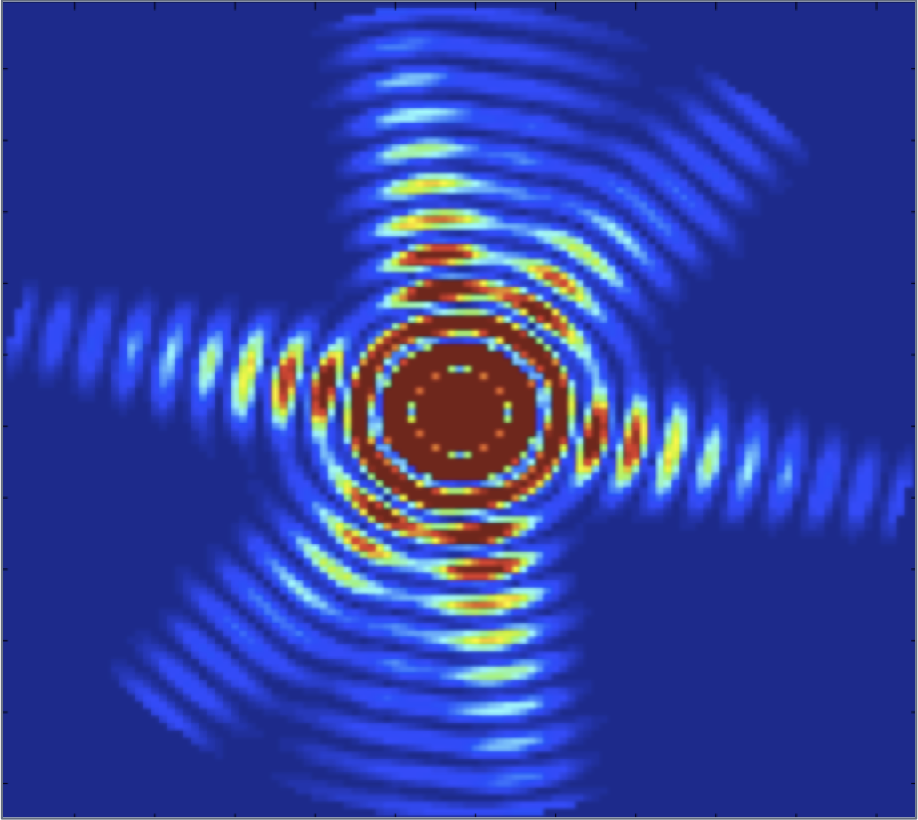
\includegraphics[width=.8\textwidth]{dppbcv}
  \caption{PBCV (Paramecium bursaria chlorella)}
\end{subfigure}
\begin{subfigure}{.5\textwidth}
  \centering
  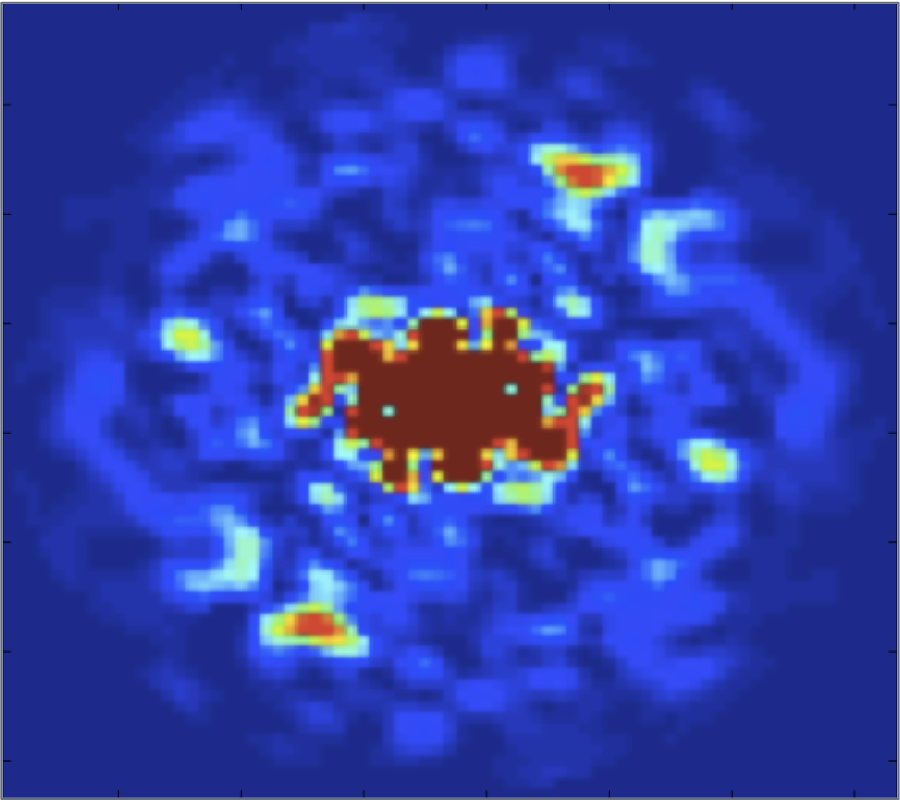
\includegraphics[width=.8\textwidth]{dppyp}
  \caption{PYP (Photoactive yellow protein)}
\end{subfigure}
\caption{A noise free diffraction pattern in random orientation}
\label{fig:simdp}
\end{figure}
Typical diffraction pattern from PBCV and PYP are displayed in figure \ref{fig:simdp}. It is easily recognized that the diffraction pattern from PBCV is from a symmetrical object whereas the diffraction pattern from PYP doesn't have an indication of symmetry. 

\begin{figure}[h]
\begin{subfigure}{.5\textwidth}
  \centering
  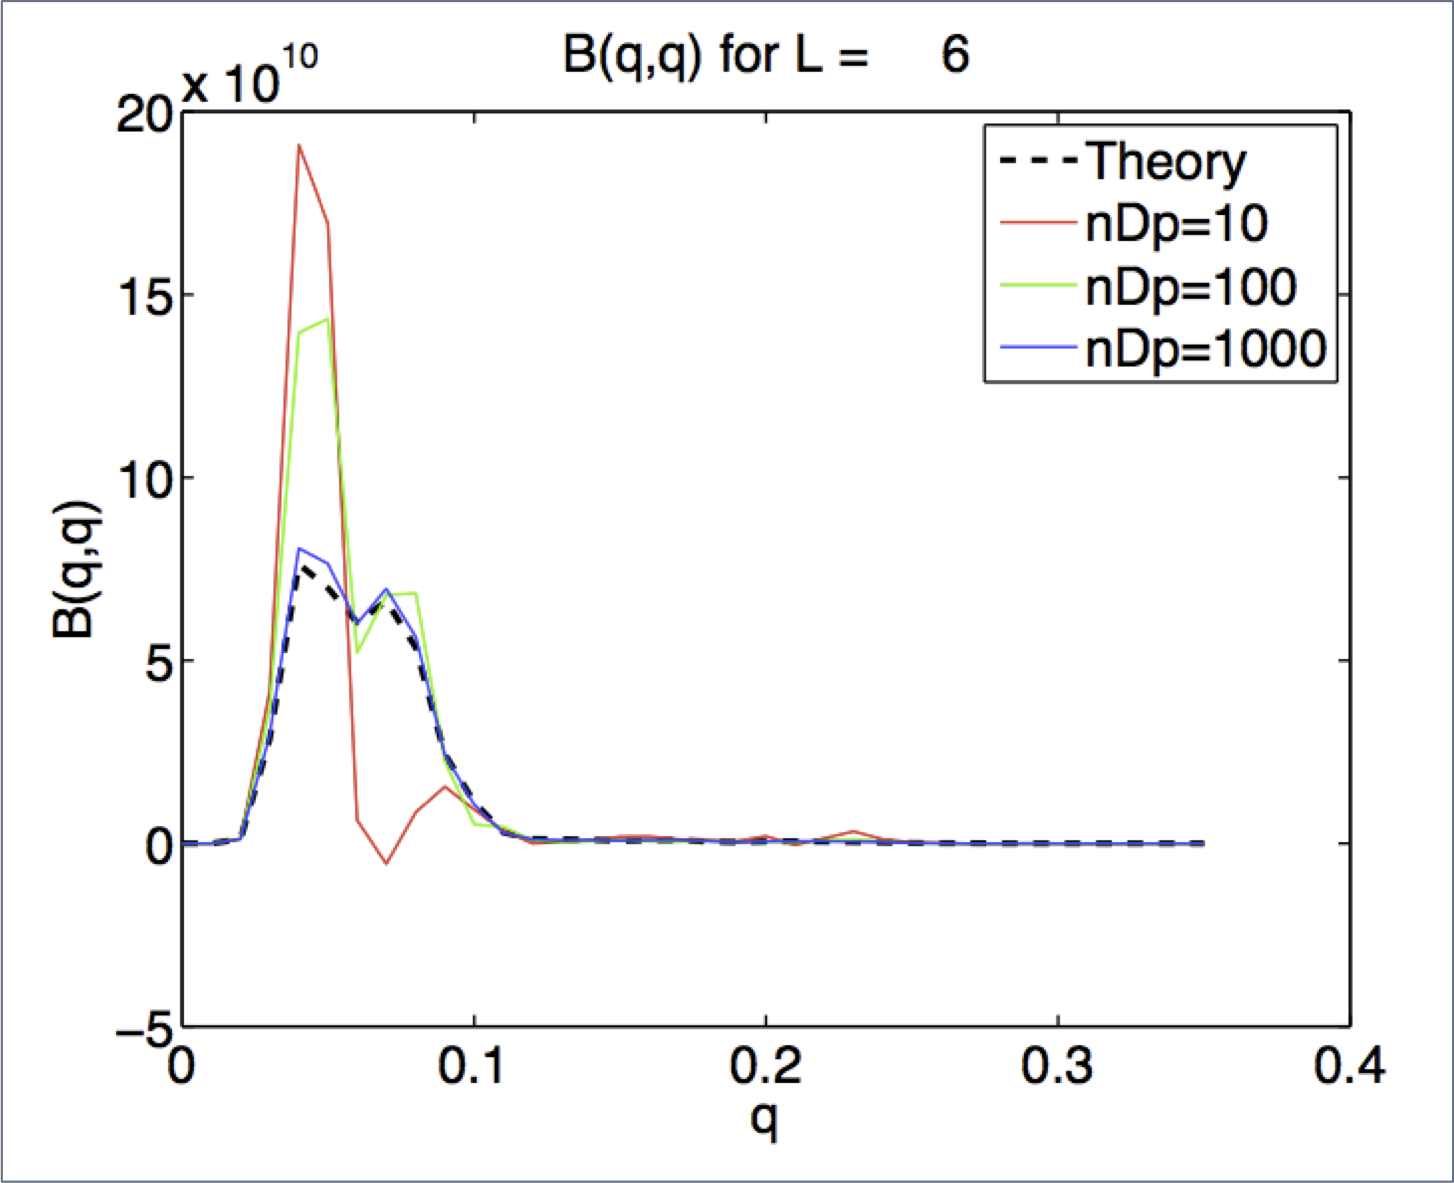
\includegraphics[width=.8\textwidth]{convpypl6}
  \caption{\Blq for $l=6$}
  \label{fig:convpypl6}
\end{subfigure}
\begin{subfigure}{.5\textwidth}
  \centering
  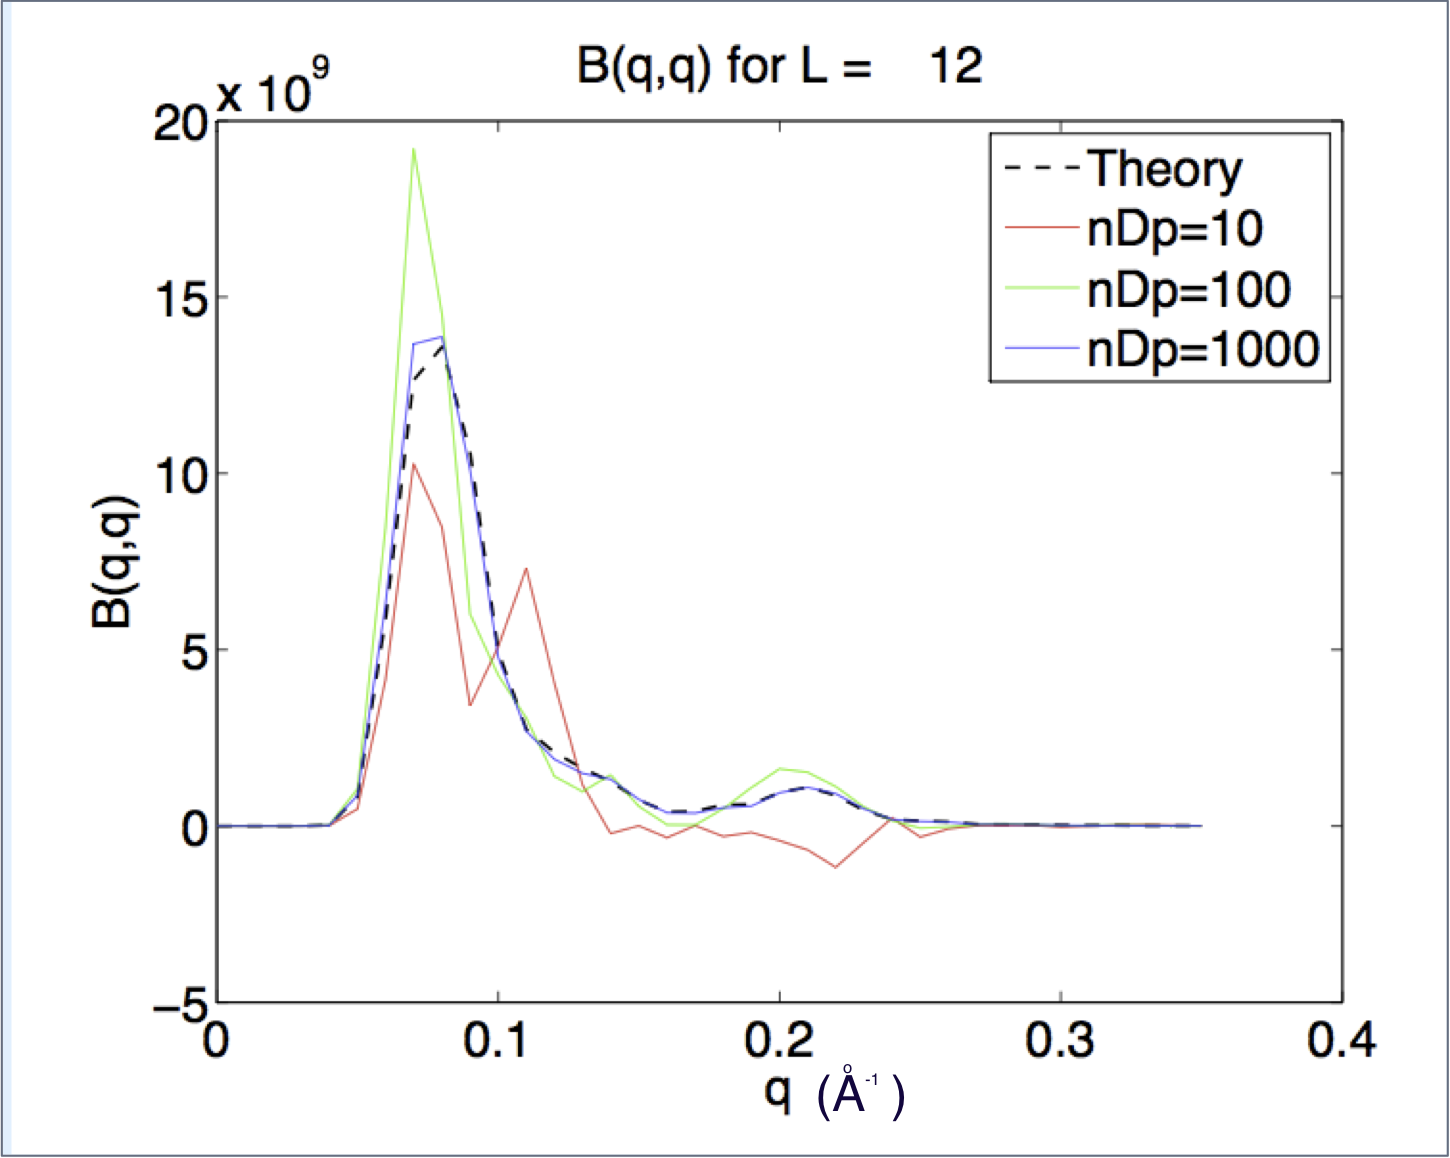
\includegraphics[width=.8\textwidth]{convpypl12}
  \caption{\Blq for $l=12$}
\end{subfigure}
\caption{Convergence of \Blq from a set of noise free diffraction patterns of PYP}
\label{fig:convpyp}
\end{figure}

The convergence of \Blq can be analyzed by comparing three different sets of simulated diffraction patterns. From figure \ref{fig:convpyp}, there are curves of \Blq that are calculated from 10, 100, and 1000 random noise free diffraction patterns. The curves are represented by solid lines. The dashed lines are the curves of \Blq calculated from infinite number of diffraction pattern. The solid lines are expected to converge into the dashed line for a large number of diffraction patterns.  

From figure \ref{fig:convpyp}, the dashed line coincides with the solid line when the number of diffraction pattern reach 1000. Two \Blq curve are calculated, one for $l=6$ and the other for $l=12$. Both of them show that the convergence is reached by only using 1000 diffraction patterns.

Eventhough the theory explicitly assume the requirement of infinite number of the diffraction patterns, the simulation shows that only 1000 diffraction patterns are enough to approximate the theoretical value of \Blq. The 1000 diffraction patterns indicate the feasibility of the correlation method to be used to recover the electron density.
\begin{figure}[h]
\begin{subfigure}{.5\textwidth}
  \centering
  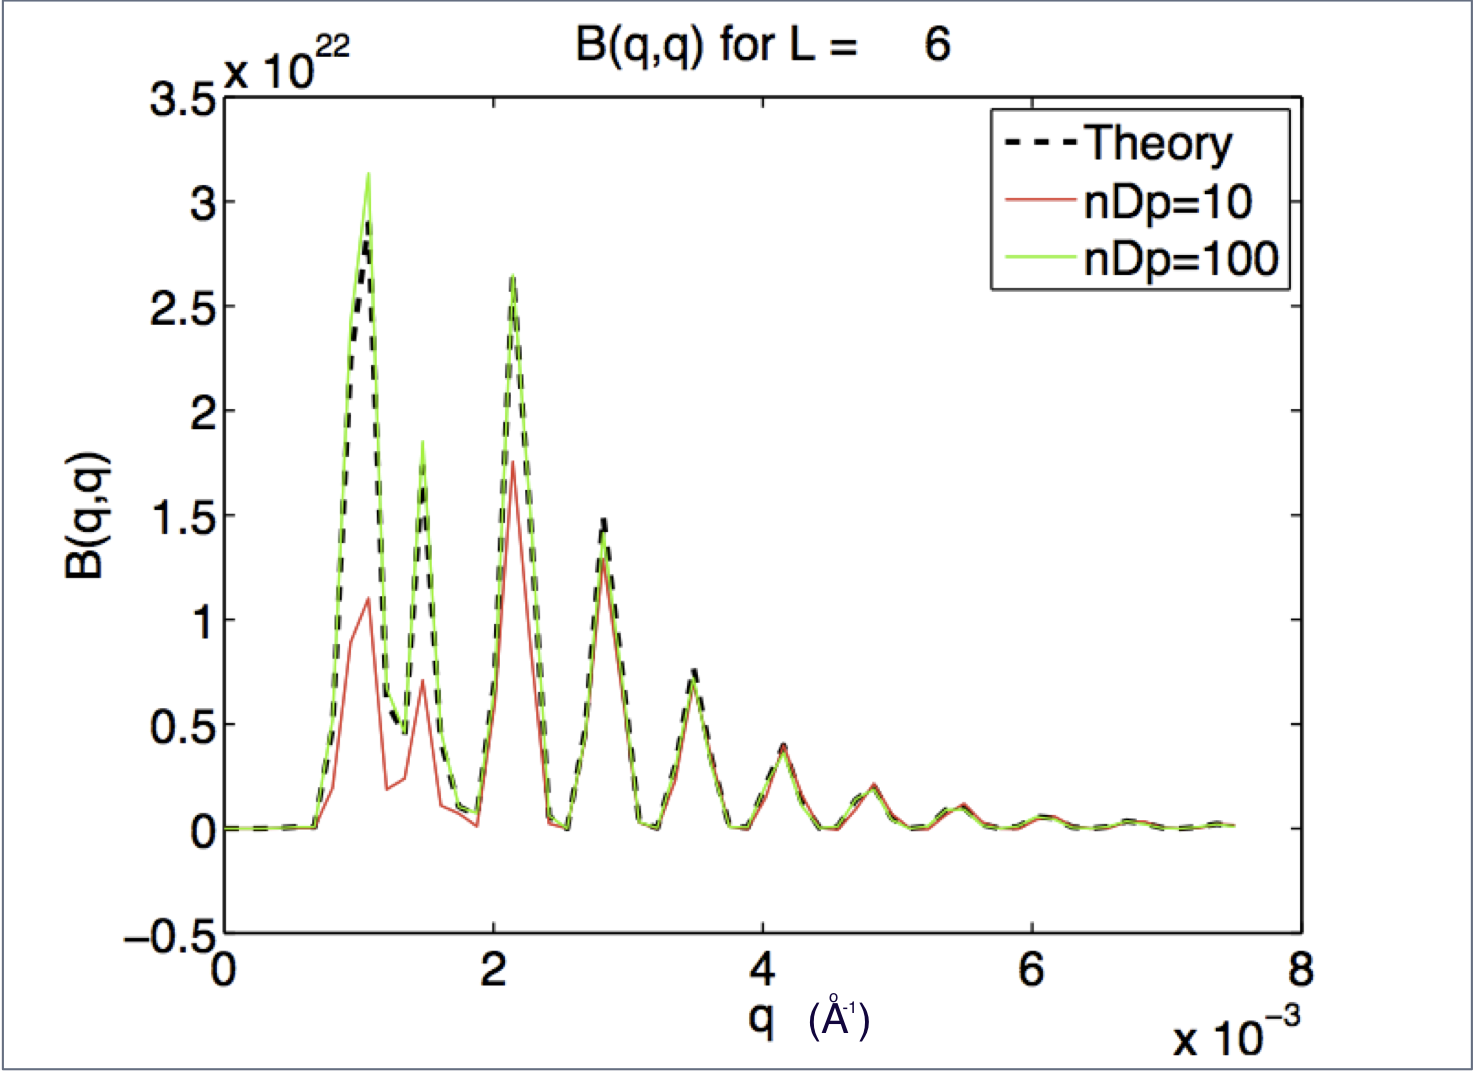
\includegraphics[width=.8\textwidth]{convpbcv6}
  \caption{\Blq for $l=6$}
  \label{fig:sub1}
\end{subfigure}
\begin{subfigure}{.5\textwidth}
  \centering
  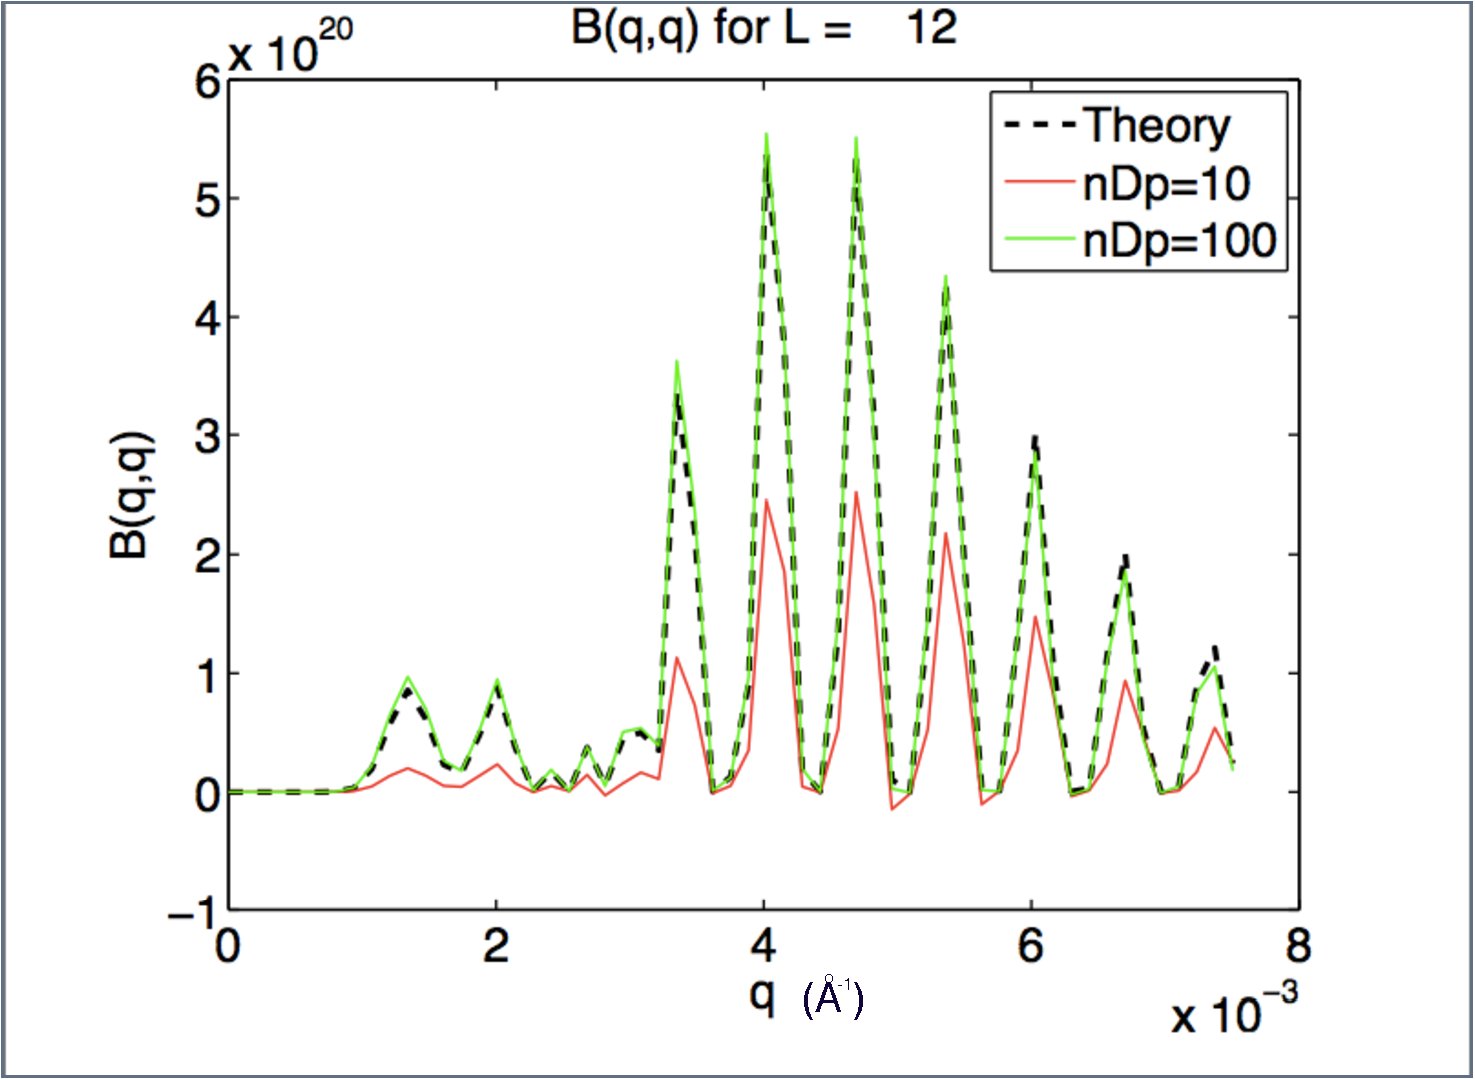
\includegraphics[width=.8\textwidth]{convpbcvl12}
  \caption{\Blq for $l=12$}
  \label{fig:sub2}
\end{subfigure}
\caption{The Convergence of \Blq from a set of noise free diffraction patterns of PBCV}
\label{fig:convpbcv}
\end{figure}

From figure \ref{fig:convpbcv}, the dashed line coincides with the solid line when number of the diffraction patterns reach 100. Two \Blq curves are calculated, one for $l=6$ and $l=25$. Both of them show the convergence is reached by only 100 diffraction patterns. In contrast to the figure \ref{fig:convpyp}, the convergence is reached by a significant smaller set of diffraction patterns. The model of figure \ref{fig:convpbcv} is PBCV, which has 60 different rotational symmetry. It is apparent from the graph that rotational symmetry reduces the total diffraction patterns needed to converge to theoretical value.     

The repetition or symmetry of particle is the reason for particle having less independent parameters. In the case of rotational symmetry, the diffraction pattern doesn't change if symmetric particle is rotated with respect to the axis of symmetry. The likelihood of having exact same diffraction pattern by rotation of random angle will increase if the particle has higher rotational symmetry. This explains the decline of the convergence of \Blq when the particle is PBCV since it has 60 rotational symmetry. 

The convergence is an important indication of properly calculated \Blq from experimental diffraction patterns. In experiment, different sets of diffraction patterns can be collected. By adding a higher number of diffraction patterns, the 2 largest set of diffraction pattern should have smaller difference because those curve nearly converge each other. It is expected that the experiment data will have higher number of diffraction patterns to converge compared to simulation. Eventhough the number of diffraction patterns needed for convergence currently is unknown for the experimental data, the convergence is necessary condition to be calculated. If convergence is not achieved, more diffraction patterns are needed for that particular structure.      

It is possible if the experimental data contain data which are dominated by noise. The inclusion of bad data in \Blq calculation will prevent the curve of \Blq vs $q$ from converging. If the portion of bad data is insignificant, it has little effect on \Blq and the convergence will be satisfied. However, whenever the bad data is significant enough in the collection of diffraction patterns, the convergence of \Blq cannot be achieved. The convergence of \Blq is important indication to observe whether bad data is present in the collection of random diffraction patterns. Provided that the convergence of \Blq is not achieved, the presence of bad data can be one of the reason therefore further effort to exclude those should be performed.

Assuming bad data is not present but convergence is not achieved, information about distribution of orientation of diffraction patterns can be deduced. Theoretically, orientation should be random or span through all angle. 
It is possible that the randomness of the orientation of the diffraction patterns is not enough to span through uniform angles. Another important point is by observing non-converging \Blq, there is possibility that the diffraction patterns have orientation tendency which is not uniform. It will give clear insight how the experiment process occur. 

This section cover the importance of the convergence of \Blq that are calculated from the collection of the diffraction patterns. The demonstration of converging \Blq is performed by using two models namely PBCV and PYP. The feasibility of the correlation method is verified by showing that only 1000 diffraction patterns of asymmetrical molecule converge into theoretical \Blq. Furthermore, the possibility of nonconverging \Blq from a set of experimental data is discussed. In conclusion, the convergence of \Blq is vital tool for analyzing experimental data and it is the first step that need to be confirmed. 


